\hypertarget{textureblitter_8cpp}{\section{/home/dave/thesis/qtwayland-\/motorcar-\/compositor/qt/src/textureblitter.cpp File Reference}
\label{textureblitter_8cpp}\index{/home/dave/thesis/qtwayland-\/motorcar-\/compositor/qt/src/textureblitter.\-cpp@{/home/dave/thesis/qtwayland-\/motorcar-\/compositor/qt/src/textureblitter.\-cpp}}
}
{\ttfamily \#include \char`\"{}textureblitter.\-h\char`\"{}}\\*
{\ttfamily \#include $<$Qt\-Gui/\-Q\-Open\-G\-L\-Shader\-Program$>$}\\*
{\ttfamily \#include $<$Qt\-Gui/\-Q\-Open\-G\-L\-Context$>$}\\*
{\ttfamily \#include $<$Qt\-Gui/\-Q\-Open\-G\-L\-Functions$>$}\\*
Include dependency graph for textureblitter.\-cpp\-:
\nopagebreak
\begin{figure}[H]
\begin{center}
\leavevmode
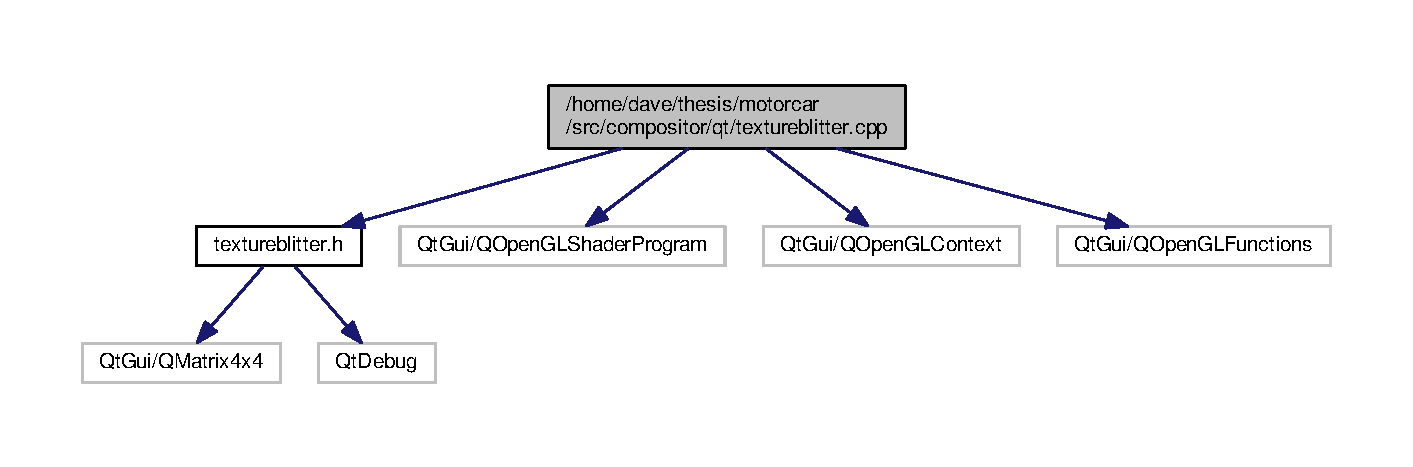
\includegraphics[width=350pt]{textureblitter_8cpp__incl}
\end{center}
\end{figure}
